\appendix
\section{Reproduction and claim--evidence map}
The source release includes synthetic interface checks, historical facade
compatibility checks, and a standalone E1 accounting verifier.
\path{REPRODUCING.md} gives the commands and expected outputs. In the E1 package,
\texttt{python -B verify.py} checks the manifest and recomputes 169 resource/cost
values from reduced records. Its ten tests run with
\texttt{python -B -m unittest}; physical-run acceptance is inherited.

The remaining \path{scripts/}, \path{docs/}, and \path{artifacts/} paths in this
supplement identify the separately retained full experiment archive. Its
\path{scripts/maxopt_v3_closeout/reverify.py} rebuilds the 36 acceptance reports,
and \path{scripts/maxopt_v3_closeout/analyze.py} generates their tables; both
require archived runs outside the compact source release. A recovery addendum restores the root environment snapshot from
identical, hash-bound per-run copies and provides a newly generated
archive integrity index. The original checksum sidecar remains
unavailable; the new index is not presented as the historical original.

\begin{itemize}[leftmargin=*]
\item Full-capacity feasibility: nine all2 reports and G-F in \path{decisions.json}.
\item Model accuracy: \path{prediction_groups.csv}, \path{common_support.csv},
      and \path{route_confusion.csv}; M1, M1b, and M2 in \path{decisions.json}.
\item H's negative result: 15 records in \path{misses.csv}; guard risk-active
      ticks and IDs in \path{guard_events.csv}.
\item Guard feasibility and cost: nine guard runs in \path{run_metrics.csv},
      with repeat-block comparisons in \path{paired_costs.csv}.
\item Production quality, physical energy, and provider billing: unsupported
      by this dataset and excluded from the claims.
\end{itemize}

\subsection{Implementation footprint}
Table~\ref{tab:implementation-footprint} separates policy logic from
integration code in the frozen execution sources. We count physical Python
lines carrying code, excluding blank lines, comments, and docstrings;
shared components are counted once. The audit records file hashes,
symbol ranges, and supporting modules, including the inherited PPO
training code. These counts describe implementation size, not historical porting effort.

\begin{table}[t]
\centering
\small
\caption{Implementation footprint in code lines. PPO policy code includes
136 lines of reused network implementation. Shared rows are separate
from the per-policy counts; backend and training dependencies are
itemized in the audit.}
\label{tab:implementation-footprint}
\setlength{\tabcolsep}{3pt}
\par\vspace{4pt}
\begin{tabular*}{\linewidth}{@{\extracolsep{\fill}}lrr@{}}
\toprule
Component & Policy & Integration\\
\midrule
B-HPA & 38 & shared\\
B-PRED & 23 & shared\\
B-MMC & 29 & shared\\
Deadline guard & 142 & 19\\
PPO & 247 & 382\\
\midrule
Shared baseline support & --- & 73\\
Shared runtime control & --- & 197\\
\bottomrule
\end{tabular*}
\end{table}

\path{IMPLEMENTATION_FOOTPRINT.json} binds these counts to the frozen
sources. The source release provides the counting script and audited
source snapshots in \path{artifact/implementation_footprint/}.

\subsection{Per-repeat latency record}
Table~\ref{tab:tail} preserves all three online tail statistics for every formal
run, from the same \texttt{run\_metrics.csv} records used in the main-text summary.

\begin{table}[h]
\centering
\fontsize{8.5}{10}\selectfont
\caption{Per-repeat online p95, p99, and maximum latency in seconds.}
\label{tab:tail}
\setlength{\tabcolsep}{2pt}
\par\vspace{4pt}
\begin{tabular*}{\linewidth}{@{\extracolsep{\fill}}lllrrr@{}}
\toprule
Policy & window & repeat & p95 & p99 & max\\
\midrule
all2 & steady & 1 & 1.598311 & 1.613852 & 1.934303 \\
all2 & steady & 2 & 1.600293 & 1.613611 & 2.053080 \\
all2 & steady & 3 & 1.598100 & 1.612091 & 2.338287 \\
all2 & recovery & 1 & 1.573470 & 1.581393 & 1.587289 \\
all2 & recovery & 2 & 1.577489 & 1.584092 & 1.587016 \\
all2 & recovery & 3 & 1.572175 & 1.582705 & 1.583298 \\
all2 & burst-offline & 1 & 1.571978 & 1.582704 & 1.673667 \\
all2 & burst-offline & 2 & 1.573614 & 1.594019 & 1.678853 \\
all2 & burst-offline & 3 & 1.567986 & 1.583607 & 1.675901 \\
all1 & steady & 1 & 2.611935 & 2.632597 & 3.617594 \\
all1 & steady & 2 & 2.606561 & 2.622125 & 3.621537 \\
all1 & steady & 3 & 2.615337 & 2.631706 & 3.626181 \\
all1 & recovery & 1 & 1.611564 & 1.626285 & 2.564877 \\
all1 & recovery & 2 & 1.616560 & 1.683677 & 2.581092 \\
all1 & recovery & 3 & 1.620432 & 1.686686 & 2.577571 \\
all1 & burst-offline & 1 & 1.647122 & 1.704174 & 1.749571 \\
all1 & burst-offline & 2 & 1.612728 & 1.632177 & 1.732826 \\
all1 & burst-offline & 3 & 1.605751 & 1.637405 & 1.729437 \\
H & steady & 1 & 17.001106 & 19.002347 & 21.001175 \\
H & steady & 2 & 17.000396 & 19.001483 & 21.001591 \\
H & steady & 3 & 17.001118 & 19.001507 & 21.002980 \\
H & recovery & 1 & 15.002311 & 15.008397 & 15.011078 \\
H & recovery & 2 & 15.002046 & 15.009679 & 15.014929 \\
H & recovery & 3 & 15.002045 & 15.008747 & 15.012199 \\
H & burst-offline & 1 & 15.003550 & 15.009867 & 15.011047 \\
H & burst-offline & 2 & 15.004760 & 15.046479 & 15.116333 \\
H & burst-offline & 3 & 15.002258 & 15.008656 & 15.009492 \\
H+guard & steady & 1 & 17.001446 & 19.002137 & 21.005507 \\
H+guard & steady & 2 & 17.001417 & 19.001712 & 21.005507 \\
H+guard & steady & 3 & 17.001367 & 19.001675 & 21.004582 \\
H+guard & recovery & 1 & 15.002007 & 15.008547 & 15.009813 \\
H+guard & recovery & 2 & 15.002468 & 15.008545 & 15.046810 \\
H+guard & recovery & 3 & 15.002523 & 15.008521 & 15.031079 \\
H+guard & burst-offline & 1 & 15.001992 & 15.003827 & 15.009511 \\
H+guard & burst-offline & 2 & 15.002109 & 15.005205 & 15.011248 \\
H+guard & burst-offline & 3 & 15.002959 & 15.024269 & 15.046434 \\
\bottomrule

\end{tabular*}
\end{table}

\subsection{Evidence provenance and scope}
The workload table is generated from \texttt{workload\_manifest.json}, whose source chain
records the 1,404,294-row BurstGPT-derived input, the parent manifest, the forward
pool selection, and the fixed thinning threshold. The selected windows have exact
prompt overlap counts of 60, 34, and 30 with their old parent windows in
steady, recovery, and burst-offline, respectively; this is disclosed as an
identity limitation rather than treated as session independence. The source has
no session field, and the offline stream is fixed synthetic pressure.

The price table is a revaluation of the same event streams over 27 price cells;
it introduces no new rollout or physical run. The guard table counts recorded
risk-active ticks, distinguishing target raises from ticks that merely maintain a
latched reservation. Two operator-aborted attempts remain in the raw history and
are excluded from the 36 formal runs; the 15 H recovery misses remain in the
formal evidence and are not replaced by guarded outcomes.

\subsection{Bridge campaign and guard audit}
The separate Bridge campaign contains 38 locked cells: an all2 capacity anchor,
two hysteresis down-threshold settings with and without the guard, and two frozen
PPO policies, each evaluated on recovery and steady windows. It is historical
evidence from a different runtime group, not an extension of the E2 pool. The
compact policy summary is shown below before the raw-event audit.

\begin{table}[t]
\centering
\small
\caption{Separate 38-cell Bridge campaign. Entries show recovery/steady P1+
counts, followed by operating cost in the same order.}
\label{tab:bridgepolicy}
\setlength{\tabcolsep}{2pt}
\par\vspace{4pt}
\begin{tabular*}{\linewidth}{@{\extracolsep{\fill}}lrrrr@{}}
\toprule
Policy & P1+ R & P1+ S & occupied R/S & cost R/S\\
\midrule
all2 (capacity anchor) & $1/1$ & $1/1$ & 4200/4200 & 4.200/4.200 \\
H-d0 & $3/3$ & $0/3$ & 1625/1778 & 1.752/2.135 \\
H-d0+guard & $3/3$ & $0/3$ & 1623/1975 & 1.752/2.314 \\
H-d1 & $0/3$ & $3/3$ & 1547/1841 & 1.709/2.208 \\
H-d1+guard & $0/3$ & $3/3$ & 1707/1837 & 1.870/2.226 \\
PPO-C30 & $1/3$ & $3/3$ & 1387/1991 & 1.626/2.075 \\
PPO-C & $0/3$ & $0/3$ & 1184/1218 & 2.547/2.935 \\
\bottomrule

\end{tabular*}
\end{table}

The Bridge guard audit joins each recorded risk ID to its request terminal and
absolute deadline; it does not rerun the policy or form a counterfactual. Each
cell below aggregates three guarded repeats. A risk-active run has at least one
nonempty risk-ID set; target raises are averaged over risk-active runs; deadline
misses count late or unfinished offline requests across the three repeats.

\begin{table}[t]
\centering
\small
\caption{Raw-event guard audit for the 12 guarded cells in the separate Bridge
campaign.}
\label{tab:bridgeguard}
\setlength{\tabcolsep}{2pt}
\par\vspace{4pt}
\begin{tabular*}{\linewidth}{@{\extracolsep{\fill}}llrrrr@{}}
\toprule
Down & window & risk runs & raises/run & misses/360 & $P1+$ pass\\
\midrule
d0 & recovery & 0/3 & 0 & 0/360 & 3/3 \\
d0 & steady & 3/3 & 2.0 & 9/360 & 0/3 \\
d1 & recovery & 3/3 & 2.0 & 7/360 & 0/3 \\
d1 & steady & 0/3 & 0 & 0/360 & 3/3 \\
\bottomrule

\end{tabular*}
\end{table}

\section{V3 accounting and gate details}
Completed requests have a completion terminal by the observation cutoff.
On-time completion includes equality with the deadline; late completion is
strictly after it. Unfinished requests lack a completed terminal at cutoff,
and missing or censored requests are not removed from the arrival denominator.
$G_F$ requires every all2 online and offline arrival on time. P1 requires
120/120 offline arrivals on time, at least 99\% of online arrivals on time,
and no unfinished request. P1+ additionally requires every online arrival
on time. These definitions follow \path{scripts/maxopt_v3/acceptance.py};
the extension's strict qualification uses the same timely/unfinished distinction.

\subsection{Replay model specification}
\label{app:replay-model-specification}
The main text lists the frozen O/C/C30/E/V parameters and controlled contrasts.
This section gives their construction and provenance. E2 reuses the frozen
C/C30 pair.

\paragraph{Service construction.}
For input length $i$, output budget $o$, and local concurrency $c$,
O assigns service duration $c(i/1024+o/128)$ seconds, using assumed rates
of 1024 input and 128 output tokens/s. C replaces this formula with the
median measured wall time per homogeneous input/output/concurrency cell.
The replay interpolates linearly in input length between 128, 512, and
2048 tokens, and in concurrency between one and four, with output budgets
restricted to 32, 128, or 256 tokens. A dedicated 256-input/256-output,
concurrency-four measurement gives 3.098\,s. Each running request accumulates
progress at the reciprocal of its current-concurrency service estimate;
this is a mixed-workload approximation, not token-level vLLM simulation.
C30, E, and V share this lookup unchanged.

\paragraph{Lifecycle construction.}
O's 30\,s startup is the original assumed constant. C's 69.219\,s proxy is
the median of 18 launch-to-ready observations collected during two-instance
initialization in nine development runs. The shared historical 7.059\,s shutdown
proxy comes from nine joint-cleanup durations; the 69.363\,s setup proxy is
the median of nine setup-barrier durations. C30 restores the 30\,s assumption
while holding C's other fields fixed; it is not a new fitted startup estimate.

The earlier empirical lifecycle model separated window restarts from setup
and normal scale-in from terminal cleanup. Medians within each run, followed
by a median across runs, gave startup/shutdown values of 25.196/1.937\,s.
V searched the nine combinations of startup multipliers
$\{0.9,1.0,1.1\}$ and shutdown multipliers $\{0.8,1.0,1.2\}$ around that
center, clipped below by the corresponding observed minima. It minimized
equal-window $L$ on the earlier development runs; leave-one-window-out and
leave-one-repeat-out checks preceded the final fit. The frozen V uses
25.196/2.325\,s and is distinct from the later $V'$ refit.

Before the held-out study, E alone was adapted to the A100 deployment:
medians from six development restarts gave 33.497/2.224\,s, followed by six
confirmation restarts. The service lookup, other models, and selected policy
were unchanged; no held-out outcomes entered this adaptation. Thus V--E
compares the historical refit with the deployment-adapted model, rather than
isolating a fitting-method effect. Windows begin with both instances ready;
the inherited setup proxy is not fitted through the window loss.
The accompanying \texttt{REPLAY\_MODEL\_SPECIFICATION.json} retains the full
lookup, unrounded parameters, and source hashes.


\subsection{Guard implementation map}
The frozen \path{scripts/maxopt_v3/policy.py} implements the following
causal projection and state update. The lookup is a conservative estimate, not a
proved upper bound, and infeasible work is still reported rather than guaranteed.
\begin{itemize}[leftmargin=*]
\item \texttt{validate\_observation} (lines 20--47) accepts only released queues,
device states, state ages, and running-job dispatch times. Future arrivals,
true readiness, and completion times are not policy inputs.
\item \texttt{duration/remaining/delay} (70--90) uses concurrency four. A running
job receives its estimated residual if positive, otherwise a full-service
fallback. Active/draining devices have zero added delay; an off device needs
the frozen safe startup time. A starting device uses the remaining safe-start
interval, then the maximum-start interval (both floored at one second), then
restarts the positive safe-start estimate if both are exceeded. A stopping
device adds remaining shutdown, or a full shutdown fallback, before startup.
\item \texttt{projected} (92--126) chooses the $k$ devices with least lifecycle
delay, with device-ID ties, and builds four slots each. Offline jobs are sorted
by deadline and ID. Without reservation, current online backlog precedes offline
work. With reservation and online backlog, offline jobs are serialized from the
earliest running offline slot, or the earliest slot if none is running. Without
online backlog they use all slots. No future arrivals are projected.
\item \texttt{decide} (128--158) first obtains H's target $b$ and intersects
latched risk IDs with pending offline IDs. It adds IDs with projected finish
$F_j(\max(1,b),r)+m+1\geq d_j$, where $m=5$ s. With active risk and scaling
enabled, it tests $k\in\{1,2\}$ using $F_j(k,r)+m\leq d_j$ for \emph{every}
pending offline job. The target is $\max(b,\min k)$ when feasible; otherwise
it is two and \texttt{infeasible} is set. A raise bypasses cooldown and updates
H's target and last-change time. Safe re-estimation alone does not clear a
latched ID; dispatch or removal from the pending queue does. Reservation is
enabled only while risk is latched and the reservation option is enabled.
\item \texttt{dispatch\_kind} (160--172) never preempts running work. With both
queues nonempty and a reservation active, an already-running offline job leaves
free slots online-first. Otherwise online takes the next slot only when its
head request's estimated slack is at most $m$ and no larger than the offline
head's slack. With no online queue, offline dispatch is unrestricted by the
single-slot reservation; without an active reservation, online has priority.
\end{itemize}

\begin{figure*}[t]
\centering
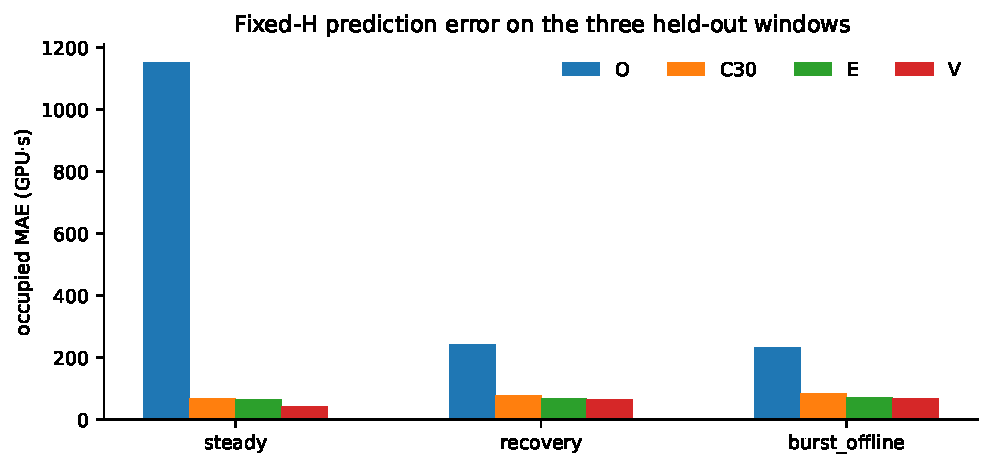
\includegraphics[width=\linewidth]{figures/fig2_model_error.pdf}
\caption{Occupied prediction error on fixed H. C30, E, and V have lower
error than O on all three windows; the main-text table also includes C.}
\end{figure*}
\begin{figure*}[t]
\centering
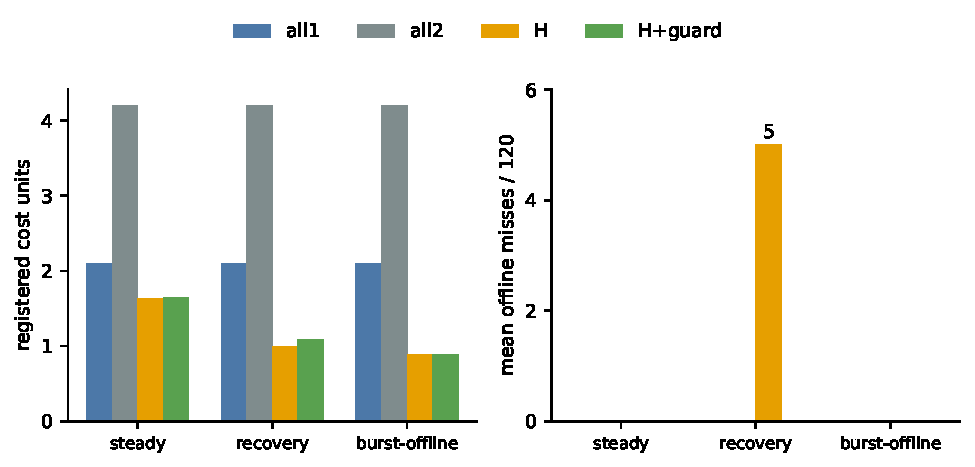
\includegraphics[width=0.96\linewidth]{figures/fig3_completion_cost.pdf}
\caption{Window cost and offline deadline misses, averaged over three repeats per
arm/window. H averages five recovery misses (15 total); all other bars are zero.
The guarded arm has no misses while reducing scenario cost relative to all1.}
\end{figure*}
\begin{table}[h]
\centering
\small
\caption{Accepted V3 cost ledger. Costs are means over three repeats;
the final two columns are savings percentages.}
\label{tab:costledger}
\setlength{\tabcolsep}{2pt}
\par\vspace{4pt}
\begin{tabular*}{\linewidth}{@{\extracolsep{\fill}}lrrrr@{}}
\toprule
Window & all1 & H+guard & window & deployment\\
\midrule
steady & 2.1029 & 1.6411 & 21.96 & 21.41 \\
recovery & 2.1029 & 1.0895 & 48.19 & 37.82 \\
burst-offline & 2.1029 & 0.8815 & 58.08 & 57.34 \\
\bottomrule

\end{tabular*}
\end{table}

\begin{table}[h]
\centering
\small
\caption{Gate interpretation for the locked V3 route; M3 is diagnostic.}
\label{tab:gates}
\setlength{\tabcolsep}{2pt}
\par\vspace{4pt}
\begin{tabular*}{\linewidth}{@{\extracolsep{\fill}}lll@{}}
\toprule
Gate & observed result & interpretation\\
\midrule
G-F & all2: 9/9 & full-capacity feasibility\\
M1 & E: 87.50\% reduction & occupied-resource gate\\
M1b & V: 34.24\% $L$ reduction & environment caveat\\
M2 & O fail; C/C30/E/V pass & matched-service fidelity\\
M3 & E: 26.77\% & diagnostic, no veto\\
P1+ & H+guard: 9/9 & online/offline feasibility\\
P2 & mean: 42.74\% & window-cost gate\\
\bottomrule
\end{tabular*}
\end{table}

\subsection{API-delay sensitivity in CPU replay}
\label{sec:api-delay-sensitivity}

We replay the four frozen rule policies (all1, all2, H, and H+guard)
on the three original windows under model E, varying only the fixed
API service delay over $\{1,2,5,10,20,40,60\}$\,s. API capacity remains
eight concurrent requests, with the same 10\,s routing wait, prices,
and policy parameters. All 12 five-second baselines reproduce the
frozen predictions, yielding 84 deterministic CPU scenarios in total.

At the tested delays of 1, 2, 5, and 10\,s, both H+guard and all1
satisfy P1+ in all three windows. Their equal-window cost savings
are 45.07\%, 45.07\%, 45.08\%, and 43.76\%, respectively.
At 20\,s, H+guard misses online deadlines in recovery and steady;
at 40 and 60\,s, online misses occur in all three guarded windows.
Longer API service occupies the finite API slots and changes
subsequent queueing, routing, and GPU control. These results test
sensitivity to the timer assumption; they are CPU predictions,
not additional physical runs or an empirical calibration of a
commercial API.

\section{V4 identity and evidence ledger}
The V4 source records supplement, rather than replace, the 36 frozen V3 runs.
Table~\ref{tab:coverage} distinguishes new execution, historical reuse, and gate
roles. All 93 accepted identities are included once; the full-strength W4's
18 gate-stopped policy cells are not counted as executions. W4-L's p075 and p050
gate batches are qualification evidence, not additional policy repeats.

\begin{table*}[t]
\centering
\small
\caption{V4 coverage and strict qualification. W4-L p050 fresh contains
all four policies; its 15/24 total must not replace their per-policy counts.}
\label{tab:coverage}
\par\vspace{4pt}
\begin{tabular*}{0.92\linewidth}{@{\extracolsep{\fill}}lrrrrl@{}}
\toprule
Workstream & fresh & reused & identities & strict & role\\
\midrule
% Generated from accepted data by scripts/maxopt_v4/paper_evidence.py.
W1 baselines & 27 & 0 & 27 & 27/27 & comparison \\
W2 Llama & 18 & 6 & 24 & 21/24 & comparison \\
W4 full load & 6 & 0 & 6 & 0/6 & gate \\
W4-L p075 gate & 6 & 0 & 6 & 0/6 & gate \\
W4-L p050 gate & 6 & 0 & 6 & 6/6 & gate \\
W4-L p050 fresh & 24 & 0 & 24 & 15/24 & comparison \\
\midrule
Total & 87 & 6 & 93 & --- & mixed roles \\
\bottomrule

\end{tabular*}
\end{table*}

Strict qualification requires at least 99\% online on-time completion,
all offline jobs completed by their deadlines, and every expected request
completed without censoring or missing work. Offline counts use each input's
actual expected denominator; formal comparison windows here contain 120 jobs,
whereas development windows may contain a different count or none.

The generated V4 rows are bound to the CPU closeout's
\path{paper_data/TABLE_MANIFEST.json}, \path{run_metrics.csv},
\path{window_summary.csv}, \path{equal_window_summary.csv}, and
\path{w4l_pairs.csv}. The source root is
\path{artifacts/max_optimization_v4_20260923/cpu_closeout_20260927/}.
Repeated requests in these CSVs are evidence about a run, not independent
replications. V3's P2 uses the equal average of within-window ratios; the W4-L
headline instead uses a ratio of equal-window means. The two statistics are
reported under their own definitions and are not numerically pooled.

\subsection{Baseline observation and selection contract}
\label{app:baselinecontract}
B-HPA updates every 60 seconds using the preceding queue observations; its
registered grid is $q_{\mathrm{target}}\in\{4,8,16\}$ and stabilization
$\in\{120,300,600\}$ seconds. B-PRED uses Holt level/trend updates with
$\alpha\in\{0.2,0.4,0.6\}$, $\beta\in\{0.1,0.3,0.5\}$, horizon
$\in\{60,120,300\}$ seconds, and margin $\in\{0,1,2\}$ (81 candidates).
B-MMC's utilization ceiling is drawn from $\{0.70,0.80,0.85,0.90\}$. Its
service lookup is shared with E to isolate the target rule; this does not provide
future information or make it an oracle. Development ranking places feasibility
before equal-window cost; the preregistered center is retained if a family has
no qualifying candidate. None of the three formal arms includes the guard.

All 9/81/4 candidates, respectively, failed development qualification. The
predeclared fallback therefore fixes B-HPA at queue target 8 and stabilization
300 seconds, B-PRED at $\alpha=0.4$, $\beta=0.3$, horizon 120 seconds and
margin 1, and B-MMC at $\rho_{\max}=0.80$. The original development feasibility
field incorrectly rejected windows containing zero offline jobs. Recalculation
with each window's actual offline denominator still leaves all 94 candidates
ineligible: each independently violates the 99\% online criterion. Thus the
fallback is unchanged, but the original field is not treated as authoritative.
The subsequent fixed-center validation repairs the preceding-60-second interval
to $[t-60,t)$ and checks the same three centers. It performs no grid search and
reads no formal or locked-test outcome; it is semantic validation, not retuning.

The runtime continuation is a comparability limitation, not an exclusion rule.
Historical W1 cells 001/002 and continuation r14 remain in the nine-per-arm
denominators. Baseline-versus-V3 comparisons are descriptive; their repeat indices
do not establish randomized pairing, and request-level resampling would not
correct the confound.

\begin{table}[t]
\centering
\small
\caption{W1 online end-to-end p99 latency (seconds): minimum--maximum
of the three completed-request per-run quantiles. These are repeat ranges, not
confidence intervals or pooled request quantiles.}
\label{tab:w1latency}
\setlength{\tabcolsep}{3pt}
\par\vspace{4pt}
\begin{tabular*}{\linewidth}{@{\extracolsep{\fill}}lrrr@{}}
\toprule
Policy & steady & recovery & burst\\
\midrule
% Generated from accepted data by scripts/maxopt_v4/paper_evidence.py.
B-HPA & 19.00--19.00 & 15.00--15.00 & 1.66--1.81 \\
B-PRED & 1.61--1.68 & 1.58--1.59 & 1.60--2.70 \\
B-MMC & 19.00--19.00 & 15.00--15.00 & 1.58--2.01 \\
\bottomrule

\end{tabular*}
\end{table}

\subsection{Failure records that constrain the claims}
\begin{table}[t]
\centering
\small
\caption{Sequential all2 qualification. Front/back list timely offline jobs
out of 120 for each of three repeats. Gates are excluded from the fresh policy
comparison.}
\label{tab:loadgate}
\setlength{\tabcolsep}{2pt}
\par\vspace{4pt}
\begin{tabular*}{\linewidth}{@{\extracolsep{\fill}}lrrrl@{}}
\toprule
Intensity & front & back & strict & action\\
\midrule
% Generated from accepted data by scripts/maxopt_v4/paper_evidence.py.
1.00 & 35/34/35 & 37/37/37 & 0/6 & stop \\
0.75 & 113/113/113 & 79/79/79 & 0/6 & lower load \\
0.50 & 120/120/120 & 120/120/120 & 6/6 & lock; fresh 24 \\
\bottomrule

\end{tabular*}
\end{table}
W2 H recovery cells 042/043 each contain 116 completed jobs out of the original
120; four unfinished jobs per cell remain in the denominator. Guard recovery
cell 049/r2 completes 120 but has only 119 timely jobs. These facts explain why
24/24 technical validity, 23/24 historical scientific acceptance, and 21/24
strict qualification are not contradictory. W2-P is not established by a
technical or historical aggregate pass.

For W4, the full-strength all2 gate stops the policy matrix after six scientific
failures. The p075 amendment gate also fails, despite eventual completion of all
offline work. The first feasible p050 gate permits, but does not substitute for,
24 fresh executions. In those fresh records H front/r1 and front/r3 each leave
two offline jobs unfinished; H back/r2 leaves four. all1's six failures remain
part of the official negative aggregate. No scientific failure is relabeled as
an operator abort, deleted, or replaced by a guarded result.

\subsection{Source and intensity provenance}
The Azure input is the conversation CSV at immutable repository commit
\path{207bed67dd10090b28ad4f745b2cfd41a11aace4}, with SHA-256
\path{2f1e5b666d4e3055fdbba98598ce2ec307767b9064e03e2fa46676dbcc7d0bf8}.
Its three columns are timestamp, context tokens, and generated tokens; only
timestamps construct the replay arrivals. The code trace is archived but not
substituted. The W4-L integer-SHA rule preserves the parent source row and
timestamp of every retained online arrival and keeps the offline stream unchanged.
Thus p050 means a locked online inclusion intensity, not half the offline work
or a rescaled time axis. Neither p050 nor the unused optional p025 is a new
independent sample of Azure production workloads.

Independent CPU checks regenerate inputs and request metrics from raw records,
and bind worker events to request identity and lifecycle generations. The
supplemental provenance package closes the three missing original-source links;
its isolated replay test suite passes 107 tests. This is verification of the
available artifact, not new GPU evidence. The original V3 convenience-snapshot
warning remains historical and is not silently rewritten.

\subsection{Time-segment cost accounting}
\begin{table}[t]
\centering
\small
\caption{W4-L 0.50 fresh comparison. Equal-window means preserve all three
repeats in each window. Only all2 and H+guard qualify strictly in all six runs.
Costs are scenario USD, not measured provider bills.}
\label{tab:w4l}
\setlength{\tabcolsep}{3pt}
\par\vspace{4pt}
\begin{tabular*}{\linewidth}{@{\extracolsep{\fill}}lrrrr@{}}
\toprule
Policy & strict & occupied & window & deployment\\
\midrule
% Generated from accepted data by scripts/maxopt_v4/paper_evidence.py.
all2 & 6/6 & 4200.0 & 4.2000 & 4.3204 \\
all1 & 0/6 & 2101.9 & 3.5248 & 3.6093 \\
H & 3/6 & 2958.9 & 3.0428 & 3.1186 \\
H+guard & 6/6 & 2992.4 & 3.0675 & 3.1366 \\
\bottomrule

\end{tabular*}
\end{table}
\begin{table}[t]
\centering
\small
\caption{W4-L p050 fresh equal-window segment means. Costs are scenario
USD; occupied time is GPU seconds. The final 600 seconds supply about 81.96\%
of guard's absolute whole-window saving against all2.}
\label{tab:segments}
\setlength{\tabcolsep}{2pt}
\par\vspace{4pt}
\begin{tabular*}{\linewidth}{@{\extracolsep{\fill}}llrrr@{}}
\toprule
Policy & seconds & occupied & cost & API cost\\
\midrule
% Generated from accepted data by scripts/maxopt_v4/paper_evidence.py.
all2 & 0--1500 & 3000.0 & 3.0000 & 0.0000 \\
all2 & 1500--1800 & 600.0 & 0.6000 & 0.0000 \\
all2 & 1800--2100 & 600.0 & 0.6000 & 0.0000 \\
all1 & 0--1500 & 1501.9 & 2.8609 & 0.5779 \\
all1 & 1500--1800 & 300.0 & 0.3639 & 0.0039 \\
all1 & 1800--2100 & 300.0 & 0.3000 & 0.0000 \\
H & 0--1500 & 2738.8 & 2.8034 & 0.0511 \\
H & 1500--1800 & 181.2 & 0.1864 & 0.0000 \\
H & 1800--2100 & 38.8 & 0.0530 & 0.0000 \\
H+guard & 0--1500 & 2728.1 & 2.7957 & 0.0536 \\
H+guard & 1500--1800 & 202.4 & 0.2081 & 0.0000 \\
H+guard & 1800--2100 & 61.9 & 0.0638 & 0.0000 \\
\bottomrule

\end{tabular*}
\end{table}
The first interval is the nominal 1,500-second source-arrival phase, not
the whole replay. The next interval still contains 20 offline arrivals per
window, and the back window's closed endpoint retains an online arrival at
1500 seconds. The $[1800,2100)$ interval extends observation through the
remaining deadline horizon. These intervals are accounting partitions, not
claims that every non-source second is empty or that the entire last 600
seconds represent a production steady state.

\section{CPU model evidence}
\subsection{W2: within-model gates and common support}
The accepted W2 analysis aligns 48 $O_x/E_x$ predictions with 24 physical
sources. It preserves the six historical all2 identities exactly once. Both
models are derived from development calibration only: $O_x$ uses a cell median
and $E_x$ a cell maximum. The simulator consumes the two-GPU aggregate lookup,
not the per-GPU metadata. Both have startup/setup 29.213463 seconds and shutdown
1.917728 seconds. Actual guarded execution uses its fixed $E_x$ plan; each
counterfactual predictor uses its corresponding model with the same policy and
safety settings. No formal outcomes fit these service or lifecycle values.

For horizon $T$, two devices, and $N$ total arrivals, the registered loss is
\begin{equation}
 L=\frac{0.5|\Delta G_{\rm occupied}|+0.25|\Delta G_{\rm active}|}{2T}
   +\frac{0.25|\Delta Q|}{TN},
\end{equation}
where $\Delta$ is prediction minus observation, $T=2100$ s for formal windows,
and $N$ includes all online and offline arrivals. $Q$ is the integrated
released-but-undispatched queue in request seconds. Unfinished jobs remain in
$N$ and contribute queue time while queued up to cutoff. Losses are averaged
over repeats within each window and then equally across windows, not over
pooled requests or matched-local support. The W3 development horizon is 900 s.
This prediction-error objective is distinct from monetary scenario cost. The W2 main
gate is $L$ reduction $\geq20\%$ on H together with per-window occupied
MAE $\leq O_x+21$ GPU seconds. The inherited occupied-improvement threshold is
a separate diagnostic, not an alternative route to a pass.

\begin{table}[t]
\centering
\small
\caption{W2 fixed-H model error; $O_x$ and $E_x$ have the same values at the
shown precision. Each window first averages its two physical repeats.}
\label{tab:w2model}
\par\vspace{4pt}
\begin{tabular*}{\linewidth}{@{\extracolsep{\fill}}lrr@{}}
\toprule
Window & $L$ (both models) & occupied MAE\\
\midrule
steady & 0.01170749 & 73.09045\\
recovery & 0.00059876 & 1.44829\\
burst-offline & 0.00032530 & 0.89862\\
equal-window & 0.00421052 & 25.14579\\
\bottomrule
\end{tabular*}
\end{table}

M2 uses the intersection of actual-GPU, $O_x$, and $E_x$ completed-local IDs.
Pairwise support is retained separately even though it coincides with common
support in these records. Fixed and dynamic M2 criteria pass, with minimum
common support 206 and maximum per-run common MAE 0.02963983 seconds. This is
not a whole-stream fidelity claim: equal-window coverage over all arrivals is
100\% for all1/all2, 51.2417\% for H, and 58.8975\% for guard. In H's two
steady repeats, only 454/457 requests are common-local, respectively, covering
29.0281\%/29.2199\% of arrivals and 53.4747\%/54.0189\% of actual-local
completions. Targets disagree with the actual controller at 1401/2100 and
1397/2100 ticks despite matching switch counts of 28. Equal-window target
disagreement is 22.2063\% for H and 0.6190\% for guard.

The zero main-metric improvement is not accidental model duplication: 14,324
requests have different $O_x/E_x$ predicted completion times. Those small
service changes do not sufficiently change the registered resource and queue
metrics. The r2 gate-only repair restores the preregistered safety conjunction;
the 48 predictions and numeric tables remain byte-identical to r1. Independent
recalculation and boundary tests accept this implementation while retaining the
scientific negative result. Evidence resides in \path{w2/decisions.json},
\path{w2/prediction_errors.csv}, \path{w2/route_confusion.csv}, and
\path{w2/target_comparison.csv} under the CPU closeout root stated above.

\subsection{W3: bounded refit and an unmet improvement gate}
The W3 development bundle contains a preformal drift record and two historical
Qwen engineering canaries (sparse and recovery), each with one observation.
Their model bytes, engine configuration, and platform match the frozen formal
deployment. The canaries contain 41 and 1440 ordinary completed GPU service
pairs, respectively; health probes are excluded. Their request IDs are disjoint
from formal IDs. These dynamic records are not independent fixed-concurrency
experiments or additional formal repeats.

A nine-cell grid varies startup by $0.9/1.0/1.1$ and shutdown by
$0.8/1.0/1.2$ around E, subject to preformal observed floors of 24.958327 and
1.897256 seconds. The development loss uses the same dimensionless definition
above at its 900-second horizon, then averages the two windows equally. The
selected $V'$ has startup 30.146928 seconds and shutdown 2.224161 seconds;
only startup differs numerically from E. Setup, the service lookup, policy,
guard model E, and all guard safety settings remain frozen. Prepare, fit, and
evaluate locks are ordered and hash-bound; formal target/event/occupied values
do not enter selection. Nevertheless, the prior V3 aggregate outcomes were
already known, so the procedure cannot be described as a new blind study.

\begin{table}[t]
\centering
\small
\caption{W3 fixed-H replay. Each window averages three physical repeats;
occupied MAE is in GPU seconds. Steady $L$ worsens. All occupied safety lines
pass, but the equal-window improvement of 5.02\% misses the 10\% gate.}
\label{tab:w3model}
\setlength{\tabcolsep}{2pt}
\par\vspace{4pt}
\begin{tabular*}{\linewidth}{@{\extracolsep{\fill}}lrrrr@{}}
\toprule
Window & E $L$ & $V'$ $L$ & E occupied & $V'$ occupied\\
\midrule
steady & 0.012390 & 0.014516 & 66.34 & 70.67\\
recovery & 0.012889 & 0.010865 & 66.95 & 66.95\\
burst-offline & 0.015303 & 0.013164 & 70.55 & 70.55\\
\bottomrule
\end{tabular*}
\end{table}

All 36 accepted formal identities enter evaluation. Twelve unique deterministic
replays per model are compared with the physical repeats, producing 72
model-by-run error records; these are not 72 new executions. E's summary,
requests, and events exactly reproduce all 12 frozen V3 prediction groups.
The primary fixed-H equal-window loss is 0.0135273755 for E and 0.0128485693
for $V'$, a reduction of 5.018019\%. The conjunctive improvement-and-safety
gate therefore fails despite three passing $E+21$ safety checks. Guard's
4.073089\% reduction is descriptive and cannot replace the primary H result;
all1/all2 are unchanged.

A technical correction in evaluation maps accepted short window names to
their full locked identifiers. It precedes prediction output and outcome
comparison, leaves the fitting grid/loss/tie-break and frozen model unchanged,
and is retained in \path{w3/evaluation_technical_amendment.json}. Independent
review reproduces the raw ledgers, selection, loss, and representative complete
simulator objects. The accepted conclusion remains negative with two-canary,
retrospective-knowledge, and lifecycle-only scope limits. Evidence includes
\path{w3/prepare/analysis_plan.json}, \path{w3/fit/frozen_model.json}, and
\path{w3/evaluate/result.json}; no new GPU run is introduced.

\section{E1: same-runtime supplementary comparison}
\label{app:e1}
E1 compares frozen H+guard and B-HPA on the previously observed
\path{locked_test_steady_v3} and \path{locked_test_recovery_v3}
inputs without revising the V3/V4 locks. All 110 formal lifecycle generations
share the two-A100 Qwen2.5-7B-Instruct FP16 runtime, model closure, service lookup,
health probe, synthetic API, and accounting contract. Both instances start
physically ready with empty queues; adapter targets remain B-HPA=0 and H+guard=2.
These targets and the intrinsic dispatch rules belong to the complete policy
treatments, so E1 does not isolate the causal contribution of the guard module.

\subsection{Identities, feasibility, and retained smoke outcomes}
The formal matrix contains one all2 capacity run per window and three fresh
repeats of each comparison policy per window: 2 capacity plus 12 comparison
identities. Each steady run contains 1,444 online and 120 offline arrivals;
each recovery run contains 334 online and 120 offline arrivals. Independent raw
recomputation finds all 14,126 formal arrivals completed on time, with zero late,
failed, or unfinished requests. Both capacity runs pass $G_F$ and every comparison
run passes P1/P1+. Table~\ref{tab:e1runs} retains all 14 identities; the capacity
runs are qualification evidence, not extra B-HPA or guard repeats.

\begin{table*}[t]
\centering
\small
\caption{All E1 formal identities. Occupied time is window GPU seconds; costs
are scenario USD. API is the percentage of all online arrivals, p99 is each
run's completed-online end-to-end quantile in seconds, and S/D counts window
starts/shutdowns. Every row completes all online and offline arrivals on time.}
\label{tab:e1runs}
\setlength{\tabcolsep}{3pt}
\par\vspace{4pt}
\begin{tabular*}{0.92\linewidth}{@{\extracolsep{\fill}}lllrrrrrr@{}}
\toprule
Window & Policy & Repeat & Occupied & Window cost & Full cost & API (\%) & p99 & S/D\\
\midrule
% Generated from independently reviewed P5_RAW_v2; see P6_TABLE_MANIFEST.json.
steady & all2 & gate & 4200.0 & 4.2000 & 4.2700 & 0.00 & 1.616 & 0/0\\
steady & B-HPA & 1 & 2407.0 & 2.4678 & 2.5389 & 6.37 & 19.002 & 2/3\\
steady & B-HPA & 2 & 2407.1 & 2.4696 & 2.5398 & 6.58 & 19.005 & 2/3\\
steady & B-HPA & 3 & 2407.2 & 2.4680 & 2.5383 & 6.37 & 19.003 & 2/3\\
steady & H+guard & 1 & 1266.0 & 1.7611 & 1.8339 & 53.25 & 19.002 & 13/15\\
steady & H+guard & 2 & 1140.5 & 1.6153 & 1.6842 & 50.83 & 19.002 & 13/15\\
steady & H+guard & 3 & 1140.3 & 1.6151 & 1.6794 & 50.83 & 19.002 & 13/15\\
recovery & all2 & gate & 4200.0 & 4.2000 & 4.2758 & 0.00 & 1.586 & 0/0\\
recovery & B-HPA & 1 & 2044.6 & 2.0715 & 2.1415 & 11.68 & 15.002 & 1/2\\
recovery & B-HPA & 2 & 2044.4 & 2.0713 & 2.1386 & 11.68 & 15.002 & 1/2\\
recovery & B-HPA & 3 & 2044.4 & 2.0713 & 2.1439 & 11.68 & 15.002 & 1/2\\
recovery & H+guard & 1 & 1102.2 & 1.2576 & 1.3279 & 60.18 & 15.008 & 12/14\\
recovery & H+guard & 2 & 794.5 & 0.9447 & 1.0110 & 58.98 & 15.008 & 11/13\\
recovery & H+guard & 3 & 794.4 & 0.9446 & 1.0104 & 58.98 & 15.008 & 11/13\\
\bottomrule

\end{tabular*}
\end{table*}

The 17 entries include three 90-second nonformal smokes.
B-HPA a1 is \texttt{TECHNICAL\_INVALID}: its lifecycle callback rejected
ready after forced stopping, leaving four offline arrivals unfinished.
After repair, a2 records 68/68 online completions on time but 0/4 offline
completions at cutoff; its \texttt{NEGATIVE\_RESULT} and false gate remain intact.
The wrapper's \texttt{PASS} denotes technical integration only.
Guard's smoke completes all 68 online and four offline arrivals on time.
None enters the formal comparison. The raw \texttt{formal\_accepted=false}
field is not overwritten; scientific qualification is independently derived from
request and lifecycle records.

\subsection{Resource use and cost boundary}
For window $w$, let $\overline C_{g,w}$ and $\overline C_{h,w}$ be the arithmetic
means across the three H+guard and B-HPA repeats. E1 reports
$R_w=1-\overline C_{g,w}/\overline C_{h,w}$ only after both arms qualify in
all three runs, then $R=(R_{\rm steady}+R_{\rm recovery})/2$.
This is the equal average of within-window ratios, not a pooled ratio or the
average of six per-pair percentages. The fixed repeat blocks support descriptive
paired differences, not confidence intervals or population-level significance.
Window scenario-cost reductions are 32.5975\% and 49.3598\%, hence 40.9786\%
equally weighted. Full-deployment reductions are 31.7650\% and 47.8629\%.

\begin{table}[t]
\centering
\small
\caption{E1 mean phase costs (scenario USD), three repeats per comparison
arm/window. Full includes setup, window, and cleanup.}
\label{tab:e1phases}
\setlength{\tabcolsep}{2pt}
\par\vspace{4pt}
\begin{tabular*}{\linewidth}{@{\extracolsep{\fill}}llrrrr@{}}
\toprule
Window & Policy & Setup & Window & Cleanup & Full\\
\midrule
% Generated from independently reviewed P5_RAW_v2; see P6_TABLE_MANIFEST.json.
steady & B-HPA & 0.0675 & 2.4685 & 0.0031 & 2.5390\\
steady & H+guard & 0.0687 & 1.6638 & 0.0000 & 1.7325\\
recovery & B-HPA & 0.0670 & 2.0714 & 0.0030 & 2.1413\\
recovery & H+guard & 0.0675 & 1.0489 & 0.0000 & 1.1164\\
\bottomrule

\end{tabular*}
\end{table}

Occupied time spans \texttt{launch\_issued} through \texttt{verified\_release},
including starting and stopping, clipped to each phase. Window occupied-time
reductions are 50.8839\% and 56.1240\%; the corresponding mean savings are
1,224.82 and 1,147.44 GPU seconds. This is local resource occupancy, not total
compute across the local and external services. Active time is not GPU compute
utilization. Guard's zero cleanup cost means that release already completed
within the window, not that release or setup is free.

Repricing the fixed ledgers makes the cost boundary explicit. Let
$\Delta C_G$, $\Delta C_A$, and $\Delta C_E$ denote mean H+guard minus
B-HPA GPU, API, and lifecycle-event costs in scenario USD.
Their steady values are $(-1.2248,0.3862,0.0340)$;
recovery gives $(-1.1474,0.0930,0.0320)$.
With GPU price multiplier $x$, a common API input/output-budget multiplier
$y$, and fixed lifecycle-event prices, the cost difference is
$\Delta C(x,y)=x\Delta C_G+y\Delta C_A+\Delta C_E$.
Neither arm incurs missed-job penalties. Since $\Delta C_A>0$, H+guard
costs less when
\[
y<y^*(x)=-\frac{x\Delta C_G+\Delta C_E}{\Delta C_A}.
\]
At $x=1$, the API break-even multipliers are 3.08 and 11.99
(3.09 and 12.02 for full deployment).
At $y=1$, window savings require GPU price multipliers above 0.343 and
0.109. Lower local GPU occupancy therefore need not imply lower cost:
the boundary depends on external-service prices. This analysis holds
routing and lifecycle events fixed, without retuning either policy.

\subsection{Routing, lifecycle, and queue trade-offs}
The online API fraction uses all online arrivals as denominator, not only local
completions. Its mean rises from 6.44\% to 51.64\% in steady and from 11.68\% to
59.38\% in recovery. Table~\ref{tab:e1tradeoffs} retains the additional lifecycle
events and queue exposure. Queue exposure sums each request's actual
release-to-dispatch time, or release-to-cutoff time if undispatched, in request
seconds. It is neither a queue-latency p99 nor a new value of the historical
prediction loss $L$. Tail latency uses completed online requests; the all-arrival
feasibility checks above independently rule out hidden formal failures.

\begin{table}[t]
\centering
\small
\caption{E1 trade-offs. S and D are mean window starts and shutdowns; Q is
mean queue request-seconds. p99 ranges span three per-run completed-online
quantiles (seconds), not confidence intervals or pooled-request quantiles.}
\label{tab:e1tradeoffs}
\setlength{\tabcolsep}{2pt}
\par\vspace{4pt}
\begin{tabular*}{\linewidth}{@{\extracolsep{\fill}}llrrrr@{}}
\toprule
Window & Policy & S & D & Q & p99 range\\
\midrule
% Generated from independently reviewed P5_RAW_v2; see P6_TABLE_MANIFEST.json.
steady & B-HPA & 2.00 & 3.00 & 1674.9 & 19.002--19.005\\
steady & H+guard & 13.00 & 15.00 & 12884.7 & 19.002--19.002\\
recovery & B-HPA & 1.00 & 2.00 & 751.1 & 15.002--15.002\\
recovery & H+guard & 11.33 & 13.33 & 9429.1 & 15.008--15.008\\
\bottomrule

\end{tabular*}
\end{table}

The two known inputs and three repeats per cell establish a bounded policy
comparison. Greater API use and queue exposure rule out all-dimensional
dominance; quality-equivalent API substitution, energy, provider bills, and
new-trace generalization remain unmeasured.

\subsection{Independent recomputation and artifact links}
The accepted table source is
\path{docs/maxopt_v4_r3_p5_20260929/ANALYSIS/P5_RAW_v2/}:
\path{FORMAL_RUNS.csv} retains 14 formal identities, \path{ATTEMPTS.csv}
all attempts, \path{PAIRS.csv} six repeat blocks, and \path{AGGREGATES.json}
the qualified estimands. \path{COMPARABILITY.json} binds plans, runtime,
and permitted policy differences. In the parent documentation directory,
\path{REVIEW_B.json} and \path{REVIEW_B_V2.json} bind accepted output hashes;
\path{P6_GENERATE_E1_TABLES.py} and \path{P6_TABLE_MANIFEST.json} reproduce
and bind the displayed rows. The standalone E1 package reproduces the resource
and price-boundary calculations from portable reduced records; its
\path{verify.py} checks the manifest and full-precision reference results.

\section{Offline decision-call microbenchmark}
This microbenchmark reuses actual states from all 16 technically valid same-runtime comparison runs, including the
B-HPA smoke with four unfinished offline jobs; the original technically invalid
a1 is excluded with its failure retained. Independent recovery matches the full
input and hidden pre/post-state of all 29,580 policy ticks, including guard
latched IDs and B-HPA's complete queue history. Remaining work is the frozen
policy's surrogate, not GPU progress inferred from future completions.

Before timing, a fixed rule chooses the earliest available tick per run and
queue stratum: empty, intermediate, or maximum observed queue size; B-HPA also
separates update and hold ticks. Empty strata stay empty. The resulting 60
snapshots are retrospective cases, not random production or held-out samples.
Each receives 100 warmup and 1,000 timed calls of the original sealed
\texttt{adapter.decide}, including its existing validation. Every call uses a
newly restored adapter and is checked against the original decision; restoration,
copying, and checks are outside \texttt{perf\_counter\_ns} timing. All 60,000
timings, including slow values, are retained; they are repeated measurements of
60 states, not 60,000 independent physical experiments.

The host is an Intel Xeon E5-2682 v4 (2.50 GHz), eight logical CPUs, with CPython
3.13.5, distinct from the GPU execution environment. CPU use is not exclusive;
affinity is unchanged and frequency policy is unavailable. Table~\ref{tab:decidecall}
reports all groups. Formal guard's largest single-snapshot p99 is 120.105
$\mu$s in steady and 92.39661 $\mu$s in recovery; its largest individual observed
times are 157.491 and 841.877 $\mu$s. The latter is retained rather than hidden
by a quantile. These are neither pooled p99s nor production-run tail estimates.

\begin{table*}[t]
\centering
\small
\caption{Offline \texttt{adapter.decide} timings, in microseconds.
Median range spans the per-snapshot medians; max p99 is the largest per-snapshot
p99, and max sample is the largest individual timing. N counts snapshots.}
\label{tab:decidecall}
\setlength{\tabcolsep}{3pt}
\par\vspace{4pt}
\begin{tabular*}{0.92\linewidth}{@{\extracolsep{\fill}}lllrrrr@{}}
\toprule
Kind & Window & Policy & N & Median range & Max p99 & Max sample\\
\midrule
% Display only: REVIEW_E2.json and P6_E2_TABLE_MANIFEST.json bind the measured source.
smoke & steady & B-HPA & 3 & 8.3695--13.0020 & 24.15627 & 36.124\\
smoke & steady & H+guard & 3 & 39.7485--45.1900 & 61.39790 & 536.644\\
capacity & steady & all2 & 3 & 2.4390--2.4660 & 2.97401 & 19.672\\
capacity & recovery & all2 & 3 & 2.3900--2.4200 & 2.97409 & 19.565\\
comparison & steady & H+guard & 9 & 43.2845--97.4360 & 120.10500 & 157.491\\
comparison & steady & B-HPA & 15 & 12.1775--30.1865 & 45.79169 & 389.906\\
comparison & recovery & B-HPA & 15 & 10.5785--25.8275 & 38.47390 & 49.562\\
comparison & recovery & H+guard & 9 & 43.3315--75.1155 & 92.39661 & 841.877\\
\bottomrule

\end{tabular*}
\end{table*}

The interval excludes \texttt{dispatch\_kind}, admission, the full controller
loop, replay/restoration, logging, I/O, worker and GPU execution. It measures
offline decision-call cost on this CPU, not complete-controller or online
end-to-end overhead, and cannot establish absence of online tail interference.
The recovery and timing sources are \path{ANALYSIS/E2_RECOVERY_v1/} and
\path{ANALYSIS/E2_BENCHMARK_v1/} under
\path{docs/maxopt_v4_r3_p5_20260929/}; the latter preserves all raw samples.
\path{REVIEW_E2.json} binds the independent audit, and
\path{P6_E2_TABLE_MANIFEST.json} binds this presentation.

\section{E2 policy evidence}
\label{app:e2policy}
The E2 handoff is independently verified by
\path{tools/verify_portable_32_cpu.py}. Its package SHA256 is
\path{079e2b7e146b1706c2500ac9a3c4a5ff0c4310885cc013907e9b86c754399aa3};
the extracted package contains 32 cells, 36 attempts, 20 strict P1+ results,
12 scientific negative results, and four retained technical-invalid attempts.
No checkpoint was retrained or selected after physical execution. The all2
reference is one cell per window; each PPO cell is a repeated execution of the
same frozen checkpoint, not a new training seed.

\begin{table*}[t]
\centering
\small
\caption{Complete E2 policy summary. Costs are means over three PPO repeats or
the single all2 anchor in each window. A negative arm can have lower cost while
still violating the strict deadline contract.}
\label{tab:e2appendix}
\setlength{\tabcolsep}{5pt}
\par\vspace{4pt}
\begin{tabular*}{0.92\linewidth}{@{\extracolsep{\fill}}llrrrrr@{}}
\toprule
Arm & training environment & R P1+ & S P1+ & cost R & cost S & offline outcome\\
\midrule
all2 & anchor & 1/1 & 1/1 & 4.200 & 4.200 & 120/120\\
C-2 & C & 0/3 & 0/3 & 2.730 & 2.950 & 4--13 on time\\
C-1 & C & 3/3 & 3/3 & 2.357 & 2.449 & 120/120\\
C30-1 & C30 & 3/3 & 3/3 & 2.073 & 2.084 & 120/120\\
C30-2 & C30 & 3/3 & 3/3 & 2.051 & 2.103 & 120/120\\
C30-3 & C30 & 0/3 & 0/3 & 1.899 & 2.090 & 106--114/120\\
\bottomrule
\end{tabular*}
\end{table*}

The physical package stores both C and C30 predictions for each cell. Comparing
the frozen prediction labels with the final physical labels gives 32/32
feasibility-direction agreement for C and 20/32 for C30. Window-cost MAE is
0.0804 and 0.4657 scenario USD, respectively; these metrics use the same
registered observation-window ledger and do not estimate provider billing.
The C30 prediction marks C30-3 feasible in both windows, while all six
physical repeats fail the offline deadline. This is a false-positive deployment
case, not a reason to remove the negative cells.

The package also retains the exact attempt history, source and tensor hashes,
request terminals, controller events, lifecycle manifests, budget receipts, and
CPU recomputation for every cell. The four technical-invalid attempts remain in
the audit trail and are excluded from scientific repeat counts. The evidence is
bounded to two locked windows, two A100 GPUs, one Qwen model, five checkpoints,
and the declared synthetic-API scenario ledger.

\subsection{Frozen PPO training and selection contract}
\label{sec:ppo-training-contract}
The capacity policy uses a 30-dimensional observation, a shared MLP with
 two 256-unit ReLU layers, three capacity logits, and a scalar value head.
The four-logit offline head is masked to its sole legal action.
Training runs in CPU replay with guard disabled, using C or C30 and
2,100-step episodes and rollouts. Adam uses learning rate $3\times10^{-4}$
and numerical epsilon $10^{-5}$; PPO uses discount $0.9995$, GAE parameter
$0.999$, clip $0.2$, four update epochs, minibatches of 64, value coefficient
$0.5$, entropy coefficient $0.01$, and gradient norm limit $0.5$.
Advantages are normalized and value loss is clipped; the learning rate
is constant. These settings are recovered from the frozen configuration,
not retuned for the deployment results.

Training uses three development windows with prefix \texttt{train\_}
and suffix \texttt{\_v2} for the burst-offline, recovery, and steady regimes.
Selection uses the corresponding three \texttt{validation\_*\_v2} windows
with deterministic C30 replay, guard disabled, and P1+ required separately
in every window. Eligible checkpoints are ordered by equal-window mean
cost, checkpoint index, and seed. E2 reuses the two previously locked
Bridge recovery and steady inputs; these are distinct files from the
selection inputs. The training contract specifies paired seeds 101--105;
Table~\ref{tab:ppo-frozen-coordinates} gives the actual selected checkpoints.
The accompanying \texttt{PPO\_TRAINING\_CONTRACT.json} records the configuration,
selection-input hashes, and checkpoint identities.
Table~\ref{tab:ppo-frozen-coordinates} maps the paper labels to the archived
identifiers. In those identifiers, \texttt{r2} denotes the second eligible
checkpoint, \texttt{s101} the seed-101/episode-40 matched pair, and
\texttt{s103} the best eligible checkpoint within seed 103; the reference
is deployed as \texttt{ppo\_C30\_raw}.

\begin{table}[t]
\centering
\small
\caption{Paper labels and frozen checkpoint identities. Steps are those
reached by the selected checkpoint. C30-2 is the registered reference.}
\label{tab:ppo-frozen-coordinates}
\setlength{\tabcolsep}{2pt}
\par\vspace{4pt}
\begin{tabular*}{\linewidth}{@{\extracolsep{\fill}}llrrr@{}}
\toprule
Label & Archive ID & Seed & Episode & Steps\\
\midrule
C-1 & C-s101 & 101 & 40 & 84,000 \\
C-2 & C-r2 & 103 & 100 & 210,000 \\
C30-1 & C30-r2 & 101 & 25 & 52,500 \\
C30-2 & C30-ref & 101 & 40 & 84,000 \\
C30-3 & C30-s103 & 103 & 75 & 157,500 \\
\bottomrule
\end{tabular*}
\end{table}

\subsection{Retrospective E2 lifecycle diagnosis}
\label{sec:e2-lifecycle-diagnosis}
We diagnose all 32 accepted physical runs and their 24 frozen C/C30
predictions without retraining or selecting new checkpoints.
The two prediction configurations differ only in startup time
(69.219\,s versus 30\,s). Window launch-to-ready time exceeds 60\,s in
196 of 218 observed generations; the median of the 30 PPO runs' startup
medians is 87.92\,s. These are descriptive lifecycle measurements,
not independent experimental replicates.

C-2 exposes the interaction with the 60\,s cooldown, which starts at a
target change rather than at readiness. In the first recovery run, its
first window restart launches at 120.01\,s, becomes ready at 223.89\,s,
and enters draining at 224.01\,s without admitting work. The matched C
prediction becomes ready at 189.22\,s and drains at 190\,s, also without
admissions. C30 becomes ready at 150\,s; although the policy proposes zero
capacity, cooldown holds one GPU until 180\,s, admitting eight offline
requests. Across all six physical C-2 runs, 72 of 73 restarts longer than
60\,s enter draining within two seconds of readiness. All 687 offline
misses are already overdue before dispatch or remain undispatched at cutoff.

The other negative checkpoint has a milder queueing failure:
60 of C30-3's 65 offline misses are overdue before dispatch, while all
requests eventually complete. Long startup alone does not imply failure:
C-1 passes despite 78 of its 84 window restarts exceeding 60\,s,
retaining capacity to clear its queues. C30-1 and C30-2 also pass,
generally keeping a worker available after restarting.
These archived trajectories explain a concrete failure pathway and why
C detects its feasibility consequence. They do not establish a general
ranking of startup models or attribute every physical timing difference
to startup alone.


\begin{figure*}[t]
\centering
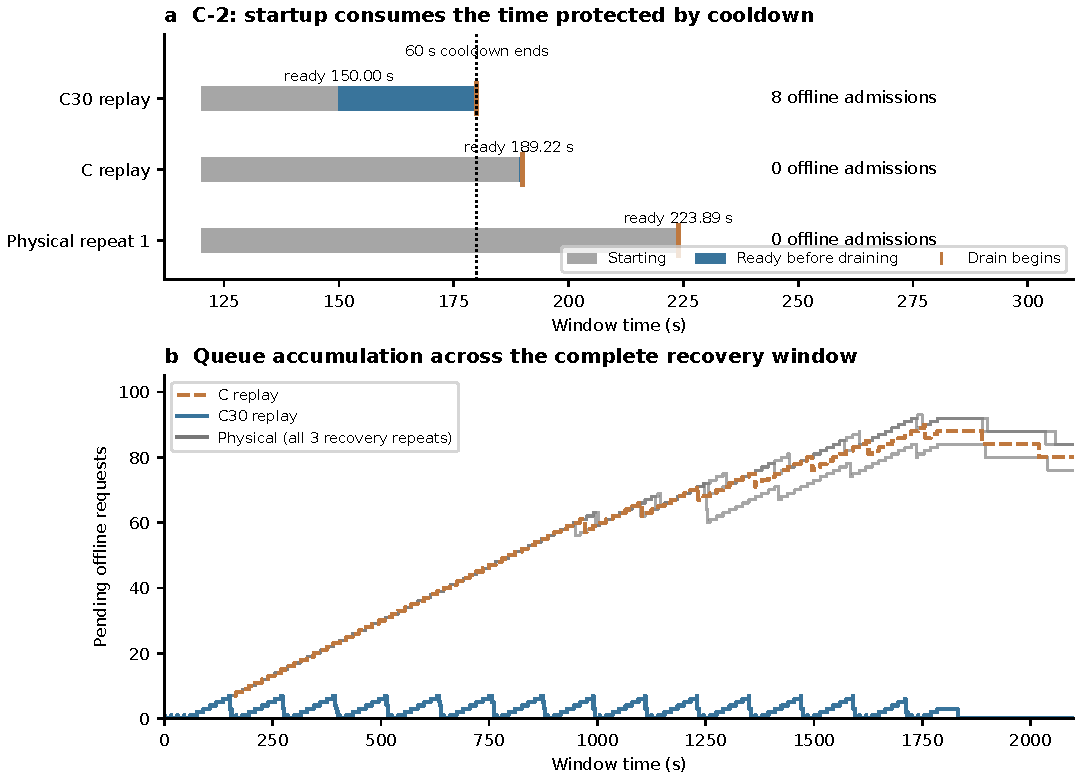
\includegraphics[width=\textwidth]{mechanism_diagnosis.pdf}
\caption{Retrospective C-2 recovery diagnosis. Top: the first window
restart of the first formal negative run and its frozen C/C30 predictions;
admissions count offline requests dispatched during that instance generation.
The dotted line marks cooldown expiry, measured from the target change.
Bottom: pending offline queues in both predictions and all three physical
recovery repeats. The text summarizes both windows and the passing-policy controls.
No new physical runs are introduced.}
\label{fig:e2-cooldown-diagnosis}
\end{figure*}

\section{Retrospective lifecycle-trajectory diagnosis}
\label{sec:v5-trajectories}
This analysis reuses all nine accepted fixed-H physical runs and the twelve
unique O/C/C30/E predictions from the frozen V3 evaluation: three windows,
three physical repeats per window, and four model comparisons per run.
The resulting 36 pairings are not new experiments or independent prediction
samples. We neither refit a model nor replace the original M1 endpoint.
The artifact binds the consumed records to their original acceptance hashes
and rechecks all 44,100 decisions across the 21 unique traces.

\subsection{Definitions and event alignment}
Time is relative to each window start, on $[0,2100)$ seconds.
Physical occupied capacity counts each generation from launch until verified
release, clipped to that interval; simulated capacity includes every non-off
state, including stopping. Let $n_m(t)$ and $n_r(t)$ be predicted and observed
occupied GPU counts. For model $m$ and repeat $r$, we distinguish
\begin{align}
A_{m,r} &= \left|\int_0^{2100}(n_m(t)-n_r(t))\,dt\right|,\\
T_{m,r} &= \int_0^{2100}|n_m(t)-n_r(t)|\,dt.
\end{align}
Both have units GPU\,$\cdot$\,s. The first is the existing total-occupation
absolute error; the second measures trajectory discrepancy without signed
temporal cancellation. We integrate the piecewise-constant records exactly,
without substituting one-second samples for continuous occupation.
Table~\ref{tab:v5-groups} reports equal-repeat means within each window;
Table~\ref{tab:v5-pairs} preserves every pairing.

Targets are compared at all 2,100 one-second decision ticks. The first
state-count difference compares the decision-time counts of active, starting,
draining/stopping, and off devices; it is not the first difference of all
hidden system state. Queue and running observations precede each decision.
Routes are compared over all arrival IDs as local, synthetic API, or
undispatched. For a request whose final routes differ, the recorded first
dispatch evidence is a retrospective locator, not a time when both eventual
routes were already known. Route differences need not follow target differences.

\subsection{An endpoint discrepancy at the cooldown boundary}
The frozen C/C30 configurations differ only in the startup endpoint.
Their first common starts and subsequent divergences are shown in
Table~\ref{tab:v5-endpoints}. C30 becomes ready after 30 s, but targets stay
equal until the 60 s cooldown expires. At that tick C remains starting;
its queue-plus-running pressure exceeds the strict up-threshold of eight,
and its target rises from one to two. C30 is ready with lower pressure and
keeps target one. Both controllers have identical target/cooldown state
before this decision; swapping the observed inputs swaps this one-step action.
This diagnoses the frozen simulator contrast, not a new physical intervention
or a replay of an alternative future trajectory. At the corresponding tick,
each of the nine physical repeats has one active device, no starting device,
and target one; that is an observational anchor.
H does not read the predictor's startup parameter, and the guard's separately
frozen safety-delay parameters are not intervened on here.

\begin{table*}[t]
\centering
\small
\caption{First C/C30 startup contrast in all three windows. Times are seconds
from window start; pressure is queued plus locally running requests. The first
target difference occurs at common start plus 60 s in each window.}
\label{tab:v5-endpoints}
\par\vspace{4pt}
\begin{tabular*}{0.92\linewidth}{@{\extracolsep{\fill}}lrrrrr@{}}
\toprule
Window & Common start & C30 ready & C ready & First target difference & Pressure C/C30\\
\midrule
% Generated from accepted V5 retrospective analysis; do not edit values.
Burst & 195 & 225 & 264.219 & 255 & 13/1\\
Recovery & 126 & 156 & 195.219 & 186 & 14/2\\
Steady & 171 & 201 & 240.219 & 231 & 21/4\\
\bottomrule

\end{tabular*}
\end{table*}

\subsection{Counterexamples and temporal cancellation}
The six burst/recovery physical repeats first differ from all four models
in target at $t=3$ s, before any window restart. At that tick the models
observe no local running request while the physical controllers still do;
completion observation has crossed a decision tick. These differences cannot
be attributed to window-restart timing. Conversely, steady repeats 1 and 3 have exactly
the same 2,100 targets as C30 despite 154 and 152 state-count difference
ticks, 48 and 45 route differences, and nonzero occupied-resource errors.
Readiness error therefore does not necessarily change a target.

The steady E total MAE is 66.34 GPU\,$\cdot$\,s, close to C30's 67.18,
but its mean trajectory error is 1,390.50 versus 114.32 GPU\,$\cdot$\,s.
The same E trace disagrees on 66.73\% of target ticks on average.
Accurate total occupation can thus hide substantial temporal mismatch;
this diagnostic does not retroactively select a different model or alter M1.
All C30 pairings retain nonzero occupation error. The largest C30 target
residual is burst repeat 2 (637/2100 ticks); its longest mismatch spans
$[1020,1144)$ s. This example is selected by an explicitly post-hoc maximum
residual rule after the full audit, alongside all no-target-change cases.
The artifact exports every window's first common-start segment for all models
and repeats, as well as the complete startup and unmatched-pair counts.

\begin{table*}[t]
\centering
\small
\caption{All window/model means over three physical repeats. Total MAE is
mean $A_{m,r}$; trajectory error is mean $T_{m,r}$, both in GPU\,$\cdot$\,s.
Target disagreement uses 2,100 ticks per pair; route disagreement uses all
arrival IDs in that window, including undispatched requests.}
\label{tab:v5-groups}
\par\vspace{4pt}
\begin{tabular*}{0.92\linewidth}{@{\extracolsep{\fill}}llrrrr@{}}
\toprule
Window & Model & Total MAE & Trajectory error & Target diff. (\%) & Route diff. (\%)\\
\midrule
% Generated from accepted V5 retrospective analysis; do not edit values.
Burst & O & 234.48 & 457.24 & 15.17 & 27.95\\
Burst & C & 847.60 & 1369.86 & 49.63 & 27.61\\
Burst & C30 & 83.08 & 268.96 & 10.33 & 15.26\\
Burst & E & 70.55 & 237.76 & 10.33 & 15.71\\
Recovery & O & 244.08 & 421.31 & 11.71 & 27.75\\
Recovery & C & 864.20 & 1302.19 & 43.92 & 35.24\\
Recovery & C30 & 78.30 & 138.31 & 3.24 & 2.20\\
Recovery & E & 66.95 & 99.02 & 3.24 & 4.19\\
Steady & O & 1151.97 & 1517.83 & 59.40 & 42.84\\
Steady & C & 964.14 & 1621.50 & 73.68 & 38.87\\
Steady & C30 & 67.18 & 114.32 & 1.03 & 4.99\\
Steady & E & 66.34 & 1390.50 & 66.73 & 49.45\\
\bottomrule

\end{tabular*}
\end{table*}

\begin{table*}[t]
\centering
\small
\caption{All 36 model/physical-repeat pairings. Errors are GPU\,$\cdot$\,s;
target differences are counts out of 2,100 ticks. A dash means targets never
differ, not a missing record. Route counts retain the full arrival denominator.
The twelve unique predictions are reused across the nine physical runs.}
\label{tab:v5-pairs}
\par\vspace{4pt}
\begin{tabular*}{0.92\linewidth}{@{\extracolsep{\fill}}llrrrrrr@{}}
\toprule
Window & Model & Rep. & Total error $A$ & Trajectory $T$ & Target diff. & First diff. (s) & Route diff./arrivals\\
\midrule
% Generated from accepted V5 retrospective analysis; do not edit values.
Burst & O & 1 & 300.54 & 304.39 & 147 & 3 & 65/297\\
Burst & O & 2 & 103.59 & 764.07 & 662 & 3 & 117/297\\
Burst & O & 3 & 299.30 & 303.26 & 147 & 3 & 67/297\\
Burst & C & 1 & 913.66 & 1347.35 & 1056 & 3 & 76/297\\
Burst & C & 2 & 716.71 & 1416.14 & 1015 & 3 & 90/297\\
Burst & C & 3 & 912.42 & 1346.08 & 1056 & 3 & 80/297\\
Burst & C30 & 1 & 53.54 & 53.54 & 7 & 3 & 2/297\\
Burst & C30 & 2 & 143.41 & 701.03 & 637 & 3 & 128/297\\
Burst & C30 & 3 & 52.30 & 52.30 & 7 & 3 & 6/297\\
Burst & E & 1 & 4.48 & 6.53 & 7 & 3 & 6/297\\
Burst & E & 2 & 201.43 & 698.53 & 637 & 3 & 122/297\\
Burst & E & 3 & 5.72 & 8.24 & 7 & 3 & 12/297\\
Recovery & O & 1 & 305.21 & 335.21 & 187 & 3 & 122/454\\
Recovery & O & 2 & 122.16 & 593.86 & 364 & 3 & 133/454\\
Recovery & O & 3 & 304.85 & 334.85 & 187 & 3 & 123/454\\
Recovery & C & 1 & 925.33 & 1233.56 & 895 & 3 & 156/454\\
Recovery & C & 2 & 742.28 & 1440.00 & 977 & 3 & 167/454\\
Recovery & C & 3 & 924.97 & 1233.01 & 895 & 3 & 157/454\\
Recovery & C30 & 1 & 52.21 & 52.21 & 9 & 3 & 10/454\\
Recovery & C30 & 2 & 130.84 & 310.86 & 186 & 3 & 11/454\\
Recovery & C30 & 3 & 51.85 & 51.85 & 9 & 3 & 9/454\\
Recovery & E & 1 & 5.81 & 8.75 & 9 & 3 & 21/454\\
Recovery & E & 2 & 188.86 & 279.36 & 186 & 3 & 16/454\\
Recovery & E & 3 & 6.17 & 8.95 & 9 & 3 & 20/454\\
Steady & O & 1 & 1193.59 & 1538.83 & 1255 & 99 & 686/1564\\
Steady & O & 2 & 1068.73 & 1475.71 & 1232 & 99 & 635/1564\\
Steady & O & 3 & 1193.58 & 1538.95 & 1255 & 99 & 689/1564\\
Steady & C & 1 & 1005.76 & 1623.09 & 1548 & 231 & 596/1564\\
Steady & C & 2 & 880.91 & 1618.33 & 1546 & 231 & 635/1564\\
Steady & C & 3 & 1005.76 & 1623.10 & 1548 & 231 & 593/1564\\
Steady & C30 & 1 & 76.70 & 76.70 & 0 & -- & 48/1564\\
Steady & C30 & 2 & 48.15 & 189.57 & 65 & 969 & 141/1564\\
Steady & C30 & 3 & 76.70 & 76.70 & 0 & -- & 45/1564\\
Steady & E & 1 & 74.18 & 1388.10 & 1400 & 232 & 784/1564\\
Steady & E & 2 & 50.68 & 1395.18 & 1404 & 232 & 755/1564\\
Steady & E & 3 & 74.17 & 1388.23 & 1400 & 232 & 781/1564\\
\bottomrule

\end{tabular*}
\end{table*}

These observations support checking lifecycle states, actions, and resource
trajectories alongside matched-service fit. Three controlled windows and nine
repeats do not establish a universal startup/cooldown law, randomized physical
causality, or a general guard guarantee. Software-observed readiness is not a
GPU-kernel timestamp, and the synthetic API retains its original quality and
billing limitations.


\section{External-validity evidence}
\label{sec:external}
The external-validity study (V4 in the artifacts) tests alternative target
rules (W1), a second model family (W2), and a second arrival source (W4) under
the same deadline and cost definitions. Each test is evaluated separately. The tables distinguish technical
validity from strict qualification: the latter keeps the original request
denominator, requires at least 99\% online on-time completion, every offline
job timely, and all requests completed without unfinished or censored work.
A late offline completion is not an unfinished request, but neither qualifies.
Table~\ref{tab:coverage} accounts for all 93 original V4 identities, including gates
and six historical reuses. E1 adds 14 separately accounted formal identities
(Section~\ref{app:e1}); requests are not independent experimental repeats.

\subsection{Alternative unguarded target rules}
The alternative-controller test (W1) asks whether unguarded rules can also
complete all work on time. B-HPA is an HPA-inspired queue-target controller with a
stabilization interval, not an implementation of Kubernetes HPA. B-PRED applies a
causal Holt queue predictor; B-MMC selects a capacity from the past arrival-rate
estimate and the frozen E service lookup. The three policies share the two-instance
limit, lifecycle semantics, one-second observation tick, and 60-second action
cooldown. None uses the V3 deadline guard, observes future arrivals, or trains a
learned scheduler. No registered development candidate qualified, so all three
use their predeclared center fallback; they are not presented as optimized
best-in-family implementations. Section~\ref{app:baselinecontract} records their
grids, locks, and semantic validation.

All three baselines complete all nine formal runs with timely online and offline
work (Table~\ref{tab:w1}). Their equal-window scenario costs are 2.2305, 4.0085,
and 2.7861, respectively. Each exceeds the historical V3 all1 reference, showing that timely completion
alone does not identify the lowest-cost policy. All three succeed without the
guard; adding the guard to these controllers remains untested. B-PRED's per-run online p99 is 1.58--2.70 seconds across these windows,
whereas B-HPA and B-MMC reach 15--19 seconds in steady/recovery. Thus the
higher-cost predictor also exposes a latency--resource trade-off;
Table~\ref{tab:w1latency} reports each window's three-repeat range.

\begin{table}[t]
\centering
\small
\caption{Alternative controllers (W1) under aligned deadline and cost definitions. Occupied time is in
GPU seconds; cost is window scenario USD. Saving is against the historical V3
all1 equal-window cost. The arms and historical reference use different runtimes.}
\label{tab:w1}
\setlength{\tabcolsep}{3pt}
\par\vspace{4pt}
\begin{tabular*}{\linewidth}{@{\extracolsep{\fill}}lrrrr@{}}
\toprule
Policy & strict & occupied & cost & saving (\%)\\
\midrule
% Generated from accepted data by scripts/maxopt_v4/paper_evidence.py.
B-HPA & 9/9 & 2199.5 & 2.2305 & -6.06 \\
B-PRED & 9/9 & 4007.5 & 4.0085 & -90.62 \\
B-MMC & 9/9 & 2752.6 & 2.7861 & -32.49 \\
\bottomrule

\end{tabular*}
\end{table}

This comparison has a runtime boundary. W1's historical cells 001/002 and its
r14 continuation belong to different runtime groups, and the new arms are not
randomized same-runtime pairs with the frozen V3 references. This deployment confound prevents a causal comparison with H+guard.

\subsection{A same-runtime supplementary comparison}
E1 addresses the runtime confound with fresh H+guard and B-HPA runs on the
known steady and recovery inputs. Both policies meet every deadline; H+guard
reduces window cost by 32.60\% and 49.36\%, respectively, while routing more
online work to the synthetic API (Table~\ref{tab:e1window}). This is a comparison
of complete policies, including their dispatch rules. Section~\ref{app:e1}
provides the shared-runtime contract, all 14 run identities, phase costs, and
resource--cost derivation.

\begin{table}[t]
\centering
\small
\caption{E1: means of three fresh repeats per arm/window; all pass P1+.
Cost is window scenario USD, and API share is percent of all online arrivals.}
\label{tab:e1window}
\setlength{\tabcolsep}{3pt}
\par\vspace{4pt}
\begin{tabular*}{\linewidth}{@{\extracolsep{\fill}}llrr@{}}
\toprule
Window & Policy & Cost & API (\%)\\
\midrule
% Generated from independently reviewed P5_RAW_v2; see P6_TABLE_MANIFEST.json.
steady & B-HPA & 2.4685 & 6.44\\
steady & H+guard & 1.6638 & 51.64\\
recovery & B-HPA & 2.0714 & 11.68\\
recovery & H+guard & 1.0489 & 59.38\\
\bottomrule

\end{tabular*}
\end{table}

The benefit depends on available latency margin and external-service prices:
lower occupancy comes with more lifecycle events and queue exposure, and the
API break-even multipliers are 3.08 and 11.99 at the registered GPU price.
These known-input results bound the guard's resource trade-off rather than
establishing performance on new workloads.

\subsection{A second model family}
The cross-model test (W2) uses Llama-3.1-8B-Instruct in bfloat16 with two independent TP1/PP1/DP1
instances. The 24-cell matrix contains six historical all2 gate cells reused
once and 18 fresh cells, with two repeats per arm and window. All 24 cells are
technically valid; the original scientific acceptance count is 23/24, whereas
the stricter request-completeness count is 21/24 (Table~\ref{tab:w2}). These
denominators answer different questions and are not interchangeable.

\begin{table}[t]
\centering
\small
\caption{W2 Llama results. Completed and timely columns aggregate offline
jobs only to expose missing or late work; 720 = six runs $\times$ 120 jobs.
Runs, not the 720 jobs, determine the strict qualification count.}
\label{tab:w2}
\setlength{\tabcolsep}{2pt}
\par\vspace{4pt}
\begin{tabular*}{\linewidth}{@{\extracolsep{\fill}}lrrrl@{}}
\toprule
Policy & strict & completed & timely & boundary\\
\midrule
% Generated from accepted data by scripts/maxopt_v4/paper_evidence.py.
all2 & 6/6 & 720/720 & 720/720 & none \\
all1 & 6/6 & 720/720 & 720/720 & none \\
H & 4/6 & 712/720 & 712/720 & 8 unfinished \\
H+guard & 5/6 & 720/720 & 719/720 & 1 late \\
\bottomrule

\end{tabular*}
\end{table}

H leaves four offline jobs unfinished in each recovery repeat (cells 042/043);
the denominators remain 120, not the 116 observed completions. The guard completes
all jobs but one recovery repeat (cell 049/r2) has only 119/120 timely offline
completions. The registered W2-P guard-feasibility claim therefore fails. H's recovery
failure recurs across families, while the guard loses its perfect on-time
record. With two repeats per arm/window, this test identifies a transfer
failure but cannot establish reliability across model families.

The within-Llama model comparison is also negative. On fixed H, $O_x$ and $E_x$
both have equal-window $L=0.00421052$ and occupied MAE 25.1458 GPU seconds:
neither improves over the other. The registered gate requires at least 20\%
$L$ reduction \emph{and} each window's occupied MAE no worse than $O_x+21$;
passing the latter does not rescue zero improvement. The inherited 20\%
occupied-improvement diagnostic also fails. These locks use development
median/max aggregate service lookups with identical lifecycle endpoints, not
a new Llama demonstration of the Qwen endpoint-adaptation gain. M2 passes on
completed-local common support (minimum 206 requests, maximum MAE 0.02964 s),
but H and guard cover only 51.24\% and 58.90\% of all arrivals on an equal-window
basis. This service-subset result does not establish whole-stream or controller
fidelity; the supplement reports coverage and target disagreement separately.

\subsection{Same-environment lifecycle refit}
W3 asks whether a bounded same-environment refit resolves the original V--E
comparison's environment caveat. It selects $V'$ by loss on two preformal
development canaries; a separate preformal drift probe constrains lifecycle
lower bounds. It freezes the model before CPU replay and evaluates all
36 existing physical records without new GPU runs. On fixed H, equal-window
$L$ falls from 0.01352738 to 0.01284857, a 5.02\% reduction below the registered
10\% threshold, while every window satisfies the occupied-MAE safety line
$V'\leq E+21$. Steady-window $L$ worsens despite the aggregate reduction.
The result is a scientific negative, not evidence that refitting has no effect.
Only lifecycle scalars are eligible for fitting; service, setup, and guard
safety remain fixed. The researchers already knew V3's aggregate results,
although the fitting code never consumed formal outcomes. This is a bounded
retrospective replay, not a newly blinded experiment, and it does not erase the
historical V--E caveat.


\subsection{Second arrival source and a load boundary}
The Azure conversation source associated with Splitwise
\citep{patel2024splitwise} contains 19,366 rows over about 58.4 minutes. W4
uses timestamps from its first and last non-overlapping 25-minute windows.
Replay uses fixed-corpus prompts and controlled token budgets, with the V3
synthetic API contract. This does not replay the original
prompt content or generated responses. The original
full-strength all2 gate is technically valid but scientifically negative in all
six runs (Table~\ref{tab:loadgate}); the other 18 planned policy cells are
\texttt{NOT\_RUN\_GATE\_STOP}, not missing successes. Equal-window mean online
timely completion is only 66.2\% (39.6--93.1\% across runs), and offline timely
completion is 29.9\%. No feasible-saving claim is made at that intensity.

The single sequential W4-L amendment fixes integer SHA thinning at online
intensities 0.75, 0.50, then optionally 0.25. It preserves retained row identities,
arrival times, deadlines, and all 120 offline jobs per window. At 0.75, all work
eventually completes, but only 113/120 front-window and 79/120 back-window offline
jobs are timely in each repeat. At 0.50, all six all2 gate runs pass: this is the
first feasible tested level. The subsequent 24 fresh runs use that locked level,
four policies, two windows, and three repeats. The six successful gate runs are
not merged into the fresh all2 denominator. The optional 0.25 level was not added.

The fresh comparison separates cheap failure from feasible saving
(Figure~\ref{fig:w4lsegments} and Table~\ref{tab:w4l}).
all1 qualifies in 0/6 runs and H in 3/6: H's front repeats
1 and 3 each censor two offline jobs, while back repeat 2 censors four. These eight unfinished jobs fail the strict completion criterion despite the
recorded \texttt{contract\_feasible} flag.
The guard qualifies in 6/6 and reduces equal-window occupied time from 4200.000
to 2992.407 GPU seconds (28.75\%), window cost from 4.2000 to 3.0675 (26.96\%),
and full-deployment cost from 4.3204 to 3.1366 (27.40\%). These percentages are
ratios of equal-window means, not averages of paired per-run percentages. The
official aggregate \texttt{NEGATIVE\_RESULT}, driven by all1, is preserved.
The time decomposition further limits the economic interpretation: guard cost
falls only 6.81\% during the first 1,500 seconds, and about 81.96\% of the
absolute whole-window saving arises in the final 600 seconds. The 26.96\%
headline must therefore not be extrapolated to sustained high-load serving
efficiency. Figure~\ref{fig:w4lsegments} makes the concentration explicit; the
supplement retains the numerical segment ledger.

\begin{figure}[t]
\centering
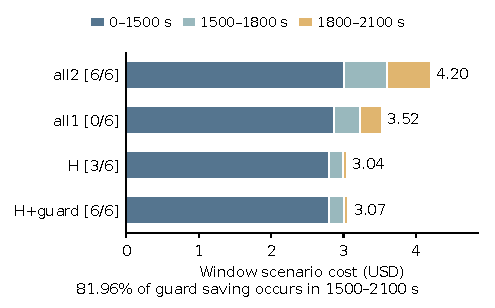
\includegraphics[width=\columnwidth]{figures/v4_w4l_segment_cost.pdf}
\caption{W4-L costs by window-time segment. Bars average three repeats per
window, then weight the two windows equally; brackets give strict passes out
of six. Lower cost in failed runs is not feasible saving. Of the guard's
saving against all2, 81.96\% occurs in the final 600 seconds.}
\label{fig:w4lsegments}
\end{figure}

Thinning reuses observed source windows; intensity was selected by the
registered all2 feasibility gate, not outcome-independent sampling. The result
is therefore load-conditioned, not a new held-out trace. Offline arrivals
continue during $[1500,1800)$, and the back window retains an online arrival
at the closed 1500-second endpoint, so source-window timing and ledger segments
are reported separately. These results do not estimate Azure's production QoS,
required fleet size, model quality, energy use, or bills.

